%----------------------------------------------------------------------------------------
%TITLE PAGE
%----------------------------------------------------------------------------------------

\begin{titlepage}

\newcommand{\HRule}{\rule{\linewidth}{0.5mm}} % Defines a new command for the horizontal lines, change thickness here


\center % Center everything on the page

\textsc{\LARGE Your university}\\[1.5cm] % Name of your university/college
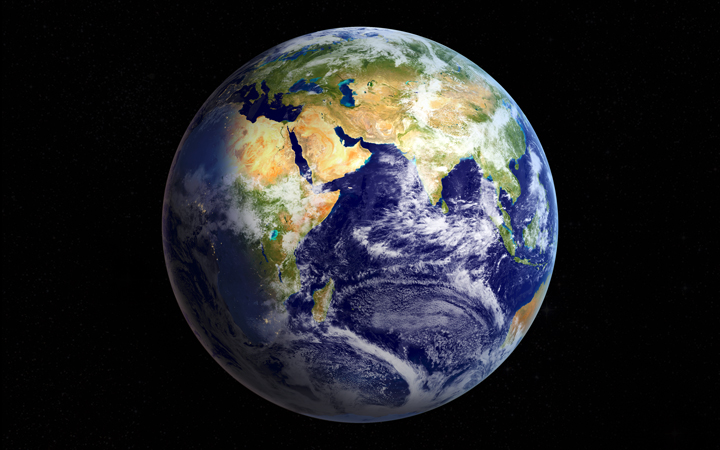
\includegraphics[width=0.5\textwidth]{earth}\par\vspace{1.5cm} % your university's logo (save it with the name logo.png in the img folder)
\textsc{\Large Your courses name or faculty name}\\[0.5cm] % Major heading such as course name
\textsc{\large More specific course name}\\[0.5cm] % Minor heading such as course title

\HRule \\[1cm]
{ \huge \bfseries Title of your report}\\[0.5cm] % Title of your document
\HRule \\[1cm]

\begin{minipage}{0.4\textwidth}
\begin{flushleft} \large
\emph{Author:}\\
Your first name \textsc{Lastname} % Your name
\end{flushleft}
\end{minipage}
~
\begin{minipage}{0.4\textwidth}
\begin{flushright} \large
\emph{Supervisor:} \\
First name \textsc{Lastname} % Supervisor's Name
\end{flushright}
\end{minipage}\\[1.5cm]

\emph{University or company address:} \\
\textsc{Name}\\
Street \\
City and zip code \\[1cm]


{\large \today}\\ % Date, change the \today to a set date if you want to be precise

\vfill % Fill the rest of the page with whitespace

\end{titlepage}
